% No preâmbulo, adicione:
% \usepackage{float}      % habilita a opção [H] (figura fixa no lugar)
% \usepackage{enumitem}   % para o label/leftmargin do enumerate
% \usepackage{graphicx}

\begin{figure}[H]
    \centering
    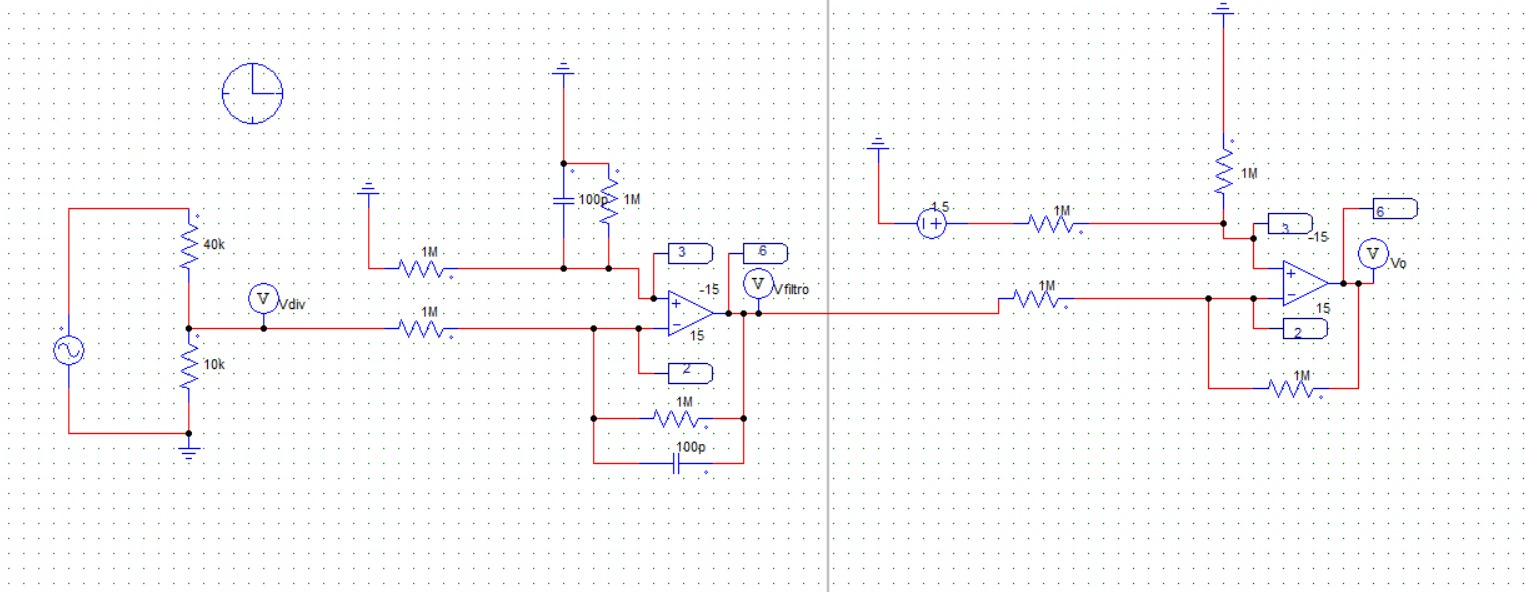
\includegraphics[width=\textwidth]{images/schematic.jpeg}
    \caption{Esquemático do circuito utilizado nas análises.}
    \label{fig:schematic}
\end{figure}

\begin{enumerate}[label=\textbf{\arabic*)}, leftmargin=*]

\item \textbf{Tensão no divisor de tensão.}
A primeira análise foi feita sobre a tensão na saída do divisor de tensão.
Esperava-se que o sinal de entrada de 5\,V fosse atenuado para uma amplitude
de 1\,V, mantendo a mesma frequência. As Figuras~\ref{fig:vdiv} e
\ref{fig:vdiv_psim} mostram, respectivamente, o resultado experimental e o
simulado no PSIM, e a Figura~\ref{fig:vsensor} apresenta a tensão do sensor.
Em ambos os casos, a tensão de saída é coerente com o esperado: a amplitude
foi reduzida para 1\,V e a frequência estabelecida foi mantida.

\begin{figure}[H]
    \centering
    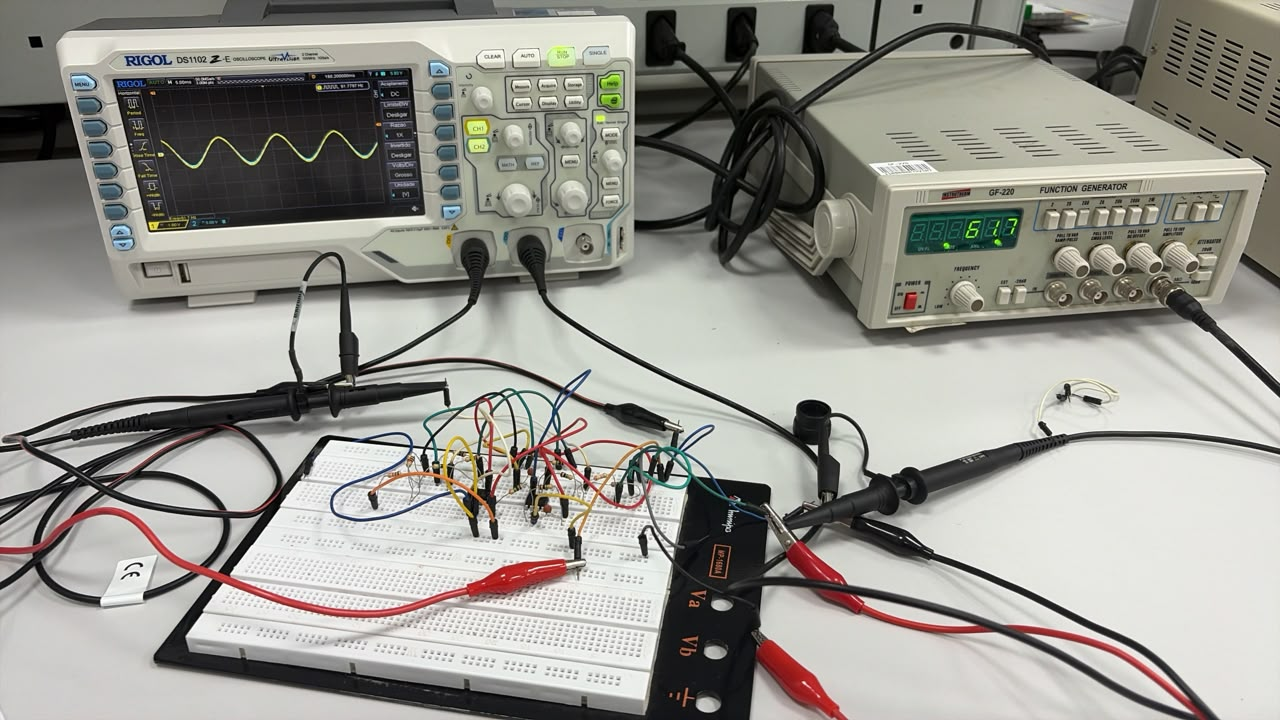
\includegraphics[width=0.9\textwidth]{images/vdiv.jpeg}
    \caption{Tensão no divisor de tensão (resultado experimental).}
    \label{fig:vdiv}
\end{figure}

\begin{figure}[H]
    \centering
    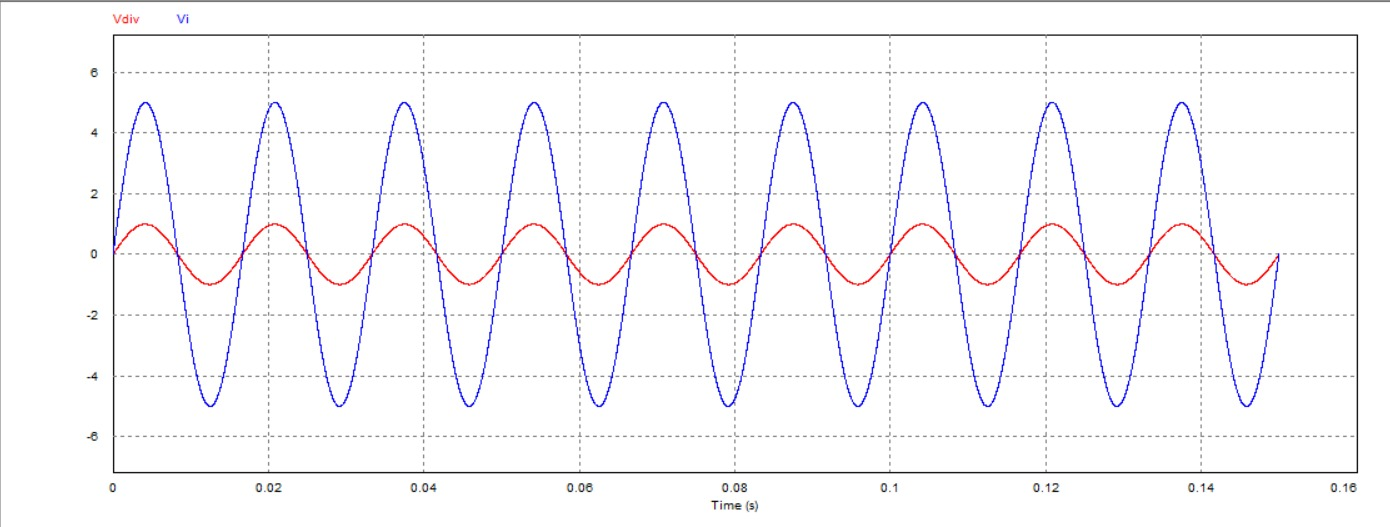
\includegraphics[width=0.9\textwidth]{images/vdiv_psim.jpeg}
    \caption{Tensão no divisor de tensão (simulação no PSIM).}
    \label{fig:vdiv_psim}
\end{figure}

\begin{figure}[H]
    \centering
    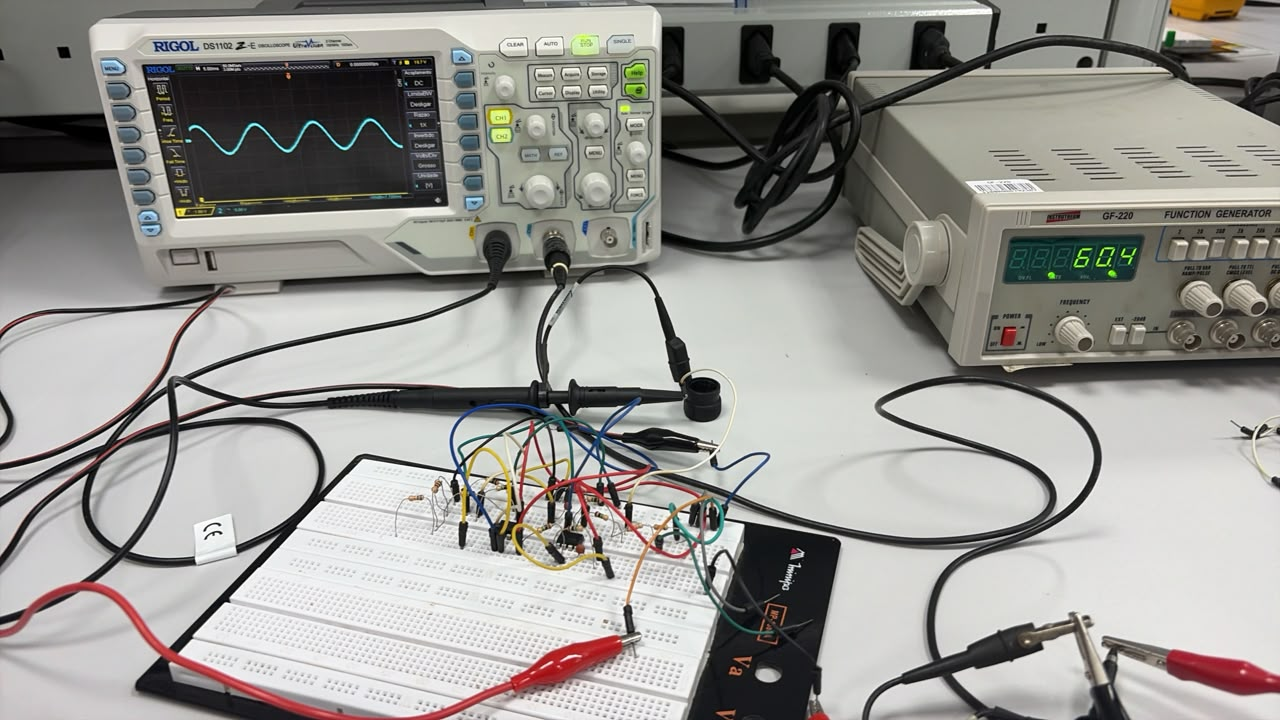
\includegraphics[width=0.9\textwidth]{images/vsensor.jpeg}
    \caption{Tensão do sensor.}
    \label{fig:vsensor}
\end{figure}

\item \textbf{Tensão na saída do filtro.}
A segunda análise foi feita sobre a saída do filtro. Esperava-se a mesma
amplitude de 1\,V, porém com o sinal invertido em relação à entrada
(defasagem de 180$^\circ$), e com a frequência mantida. Conforme as
Figuras~\ref{fig:vfiltro} e \ref{fig:vfiltro_psim}, o comportamento
observado no experimento e na simulação atende ao esperado.

\begin{figure}[H]
    \centering
    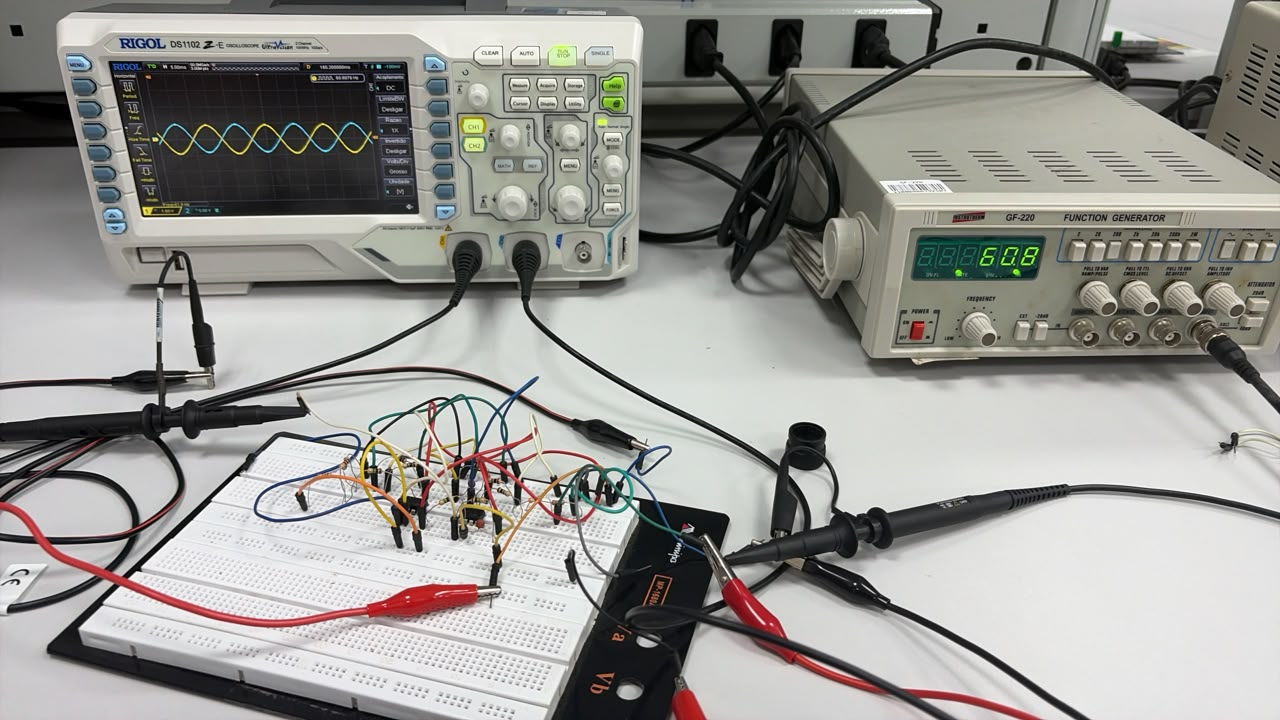
\includegraphics[width=0.9\textwidth]{images/vfiltro.jpeg}
    \caption{Tensão na saída do filtro (resultado experimental).}
    \label{fig:vfiltro}
\end{figure}

\begin{figure}[H]
    \centering
    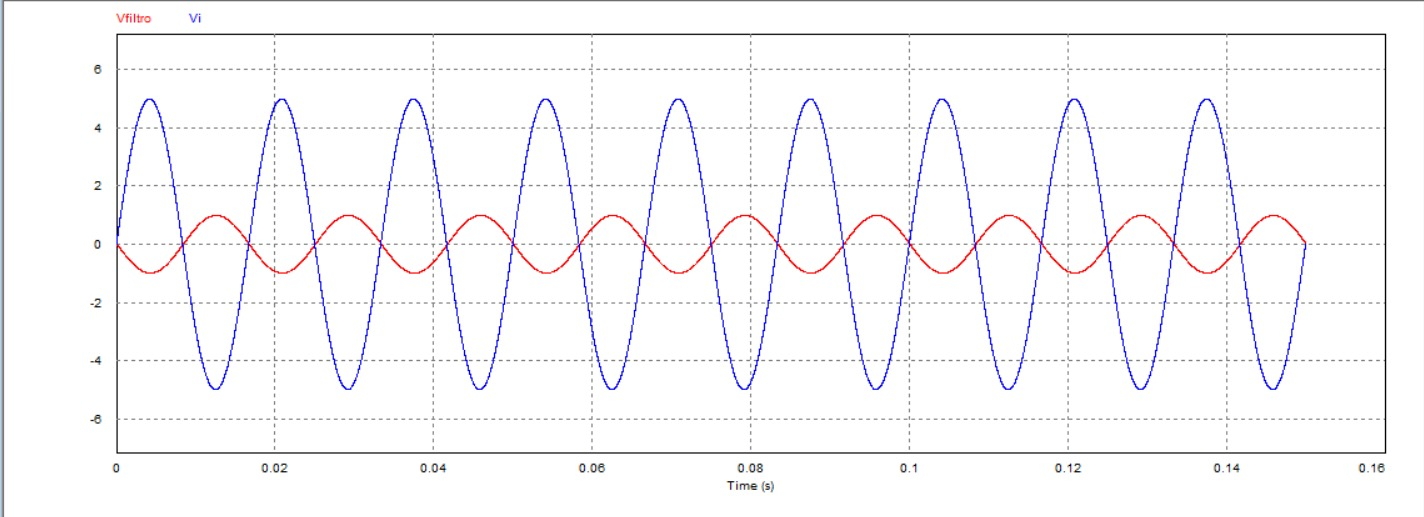
\includegraphics[width=0.9\textwidth]{images/vfiltro_psim.jpeg}
    \caption{Tensão na saída do filtro (simulação no PSIM).}
    \label{fig:vfiltro_psim}
\end{figure}

\item \textbf{Tensão de saída.}
A última análise foi feita sobre a tensão de saída do circuito.
Esperava-se que a amplitude de 1\,V fosse mantida, porém com um nível CC
(\emph{offset}) de 1,5\,V, de modo que o sinal variasse entre 0,5\,V e
2,5\,V, com a frequência inalterada. Esse deslocamento deve-se ao divisor
de tensão na entrada não inversora do último amplificador operacional.
Os resultados das Figuras~\ref{fig:vo} e \ref{fig:vo_psim} confirmam esse
comportamento.

\begin{figure}[H]
    \centering
    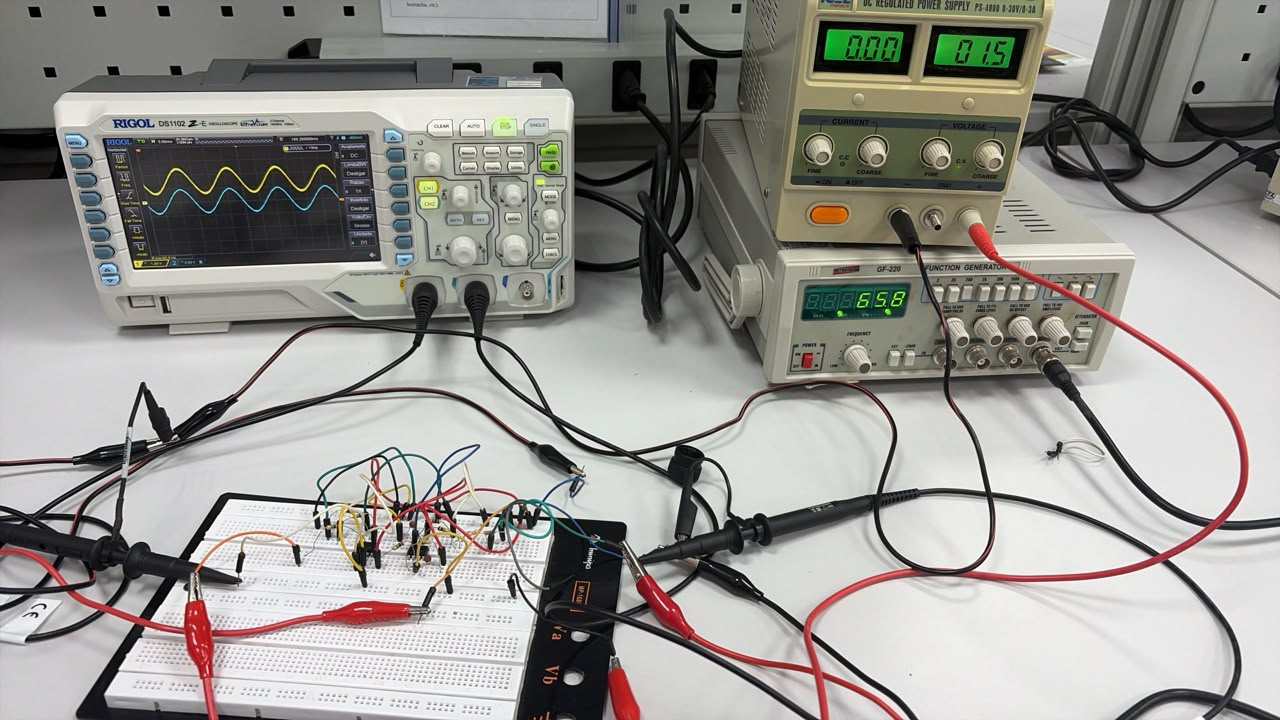
\includegraphics[width=0.9\textwidth]{images/vo.jpeg}
    \caption{Tensão de saída (resultado experimental).}
    \label{fig:vo}
\end{figure}

\begin{figure}[H]
    \centering
    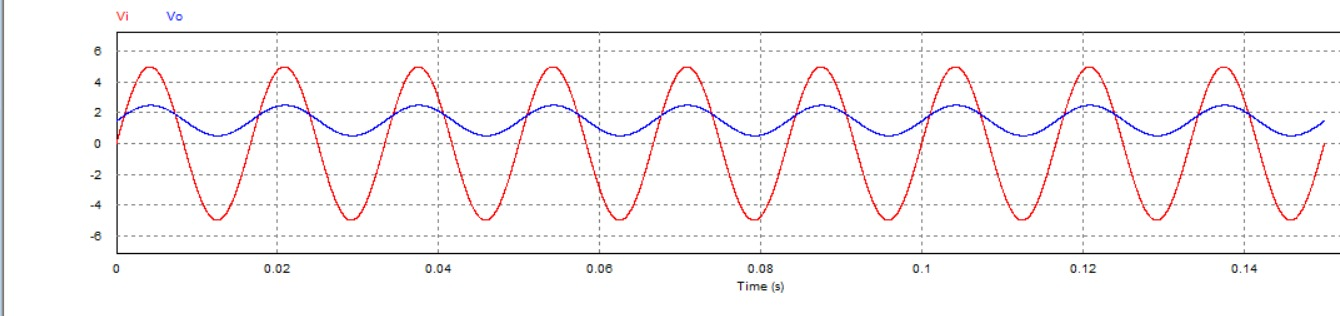
\includegraphics[width=0.9\textwidth]{images/vo_psim.jpeg}
    \caption{Tensão de saída (simulação no PSIM).}
    \label{fig:vo_psim}
\end{figure}

\end{enumerate}